
\begin{lemma}{7.2.300}\label{lem:7-2-300}
\par\noindent\textbullet\quad
可以选取 $S([0,1]_s\times L'_1)$ 的子复形
\[
\begin{gathered}
C([0,1]_s\times L'_1,\lambda'_1),\qquad
C([0,1]_s\times L'_1,(\lambda'_0,\lambda'_1)),\\
C_a([0,1]_s\times L'_1,((\lambda_0,\lambda'_0),\lambda'_1)),
\end{gathered}
\]
在它们上面选取滤过 $A_{n',K'}$ 结构，
并选取 $\operatorname{Eval}$ 与 $\operatorname{Incl}$，
使这三个复形分别成为下列对象的模型：
\[
\begin{gathered}
[0,1]_s\times C(L'_1,\lambda'_1),\qquad
[0,1]_s\times C(L'_1,(\lambda'_0,\lambda'_1)),\\
[0,1]_s\times
\bigl(C(L'_1,\lambda'_1),
\{C_a^{s=s_0}
(L'_1,((\lambda_0,\lambda'_0),\lambda'_1))\}_{s_0}\bigr).
\end{gathered}
\]
这里的“模型”指
定义~\ref{def:7-2-174} 意义下、
属于 $A_{n',K'}$ 类的模型。

\par\noindent\textbullet\quad
可以选取 $S([0,1]_s\times L'_0)$ 的子复形
\[
C([0,1]_s\times L'_0,\lambda'_0),\qquad
C([0,1]_s\times L'_0,(\lambda_0,\lambda'_0)),
\]
在它们上面选取滤过 $A_{n,K}$ 结构，
并选取 $\operatorname{Eval}$ 与 $\operatorname{Incl}$，
使这两个复形分别成为下列对象的模型：\translatornote{原书在第二个模型的端点族中把
$(\lambda_0,\lambda'_0)$ 写作
$(\lambda,\lambda'_0)$；
本项已定义的参数与图式 7.2.18
均为 $\lambda_0$，故补下标。
原书前一行还多排一个右括号。}
\[
\begin{gathered}
[0,1]_s\times C(L'_0,\lambda'_0),\\
[0,1]_s\times
\bigl(C(L'_0,\lambda'_0),
\{C^{s=s_0}(L'_0,(\lambda_0,\lambda'_0))\}_{s_0}\bigr).
\end{gathered}
\]
这里的“模型”同样指
定义~\ref{def:7-2-174} 意义下、
属于 $A_{n,K}$ 类的模型。

\par\noindent\textbullet\quad
存在滤过 $A_{n,K}$ 同态
\[
\begin{gathered}
\mathfrak f^{\operatorname{id}\times\phi'}\colon
C([0,1]_s\times L'_0,\lambda'_0)
\longrightarrow
C([0,1]_s\times L'_1,(\lambda'_0,\lambda'_1)),\\
\mathfrak f^{\operatorname{id}\times\phi'}_{\mathrm{ext}}\colon
C([0,1]_s\times L'_0,(\lambda_0,\lambda'_0))
\longrightarrow
C_a([0,1]_s\times L'_1,((\lambda_0,\lambda'_0),\lambda'_1)).
\end{gathered}
\]

\par\noindent\textbullet\quad
它们满足下列性质：

\begin{equation}
\operatorname{Eval}_{s=s_0}\circ
\mathfrak f^{\operatorname{id}\times\phi'}
=\mathfrak f^{\phi'}\circ
\operatorname{Eval}_{s=s_0}.
\tag{7.2.301.1}\label{eq:7-2-301-1}
\end{equation}
\begin{equation}
\operatorname{Eval}_{s=s_0}\circ
\mathfrak f^{\operatorname{id}\times\phi'}_{\mathrm{ext}}
=\mathfrak f^{\phi'}_{\mathrm{ext},s=s_0}\circ
\operatorname{Eval}_{s=s_0}.
\tag{7.2.301.2}\label{eq:7-2-301-2}
\end{equation}
\begin{equation}
\begin{aligned}
C([0,1]_s\times L'_1,\lambda'_1)
&\subset
C([0,1]_s\times L'_1,(\lambda'_0,\lambda'_1))\\
&\subset
C_a([0,1]_s\times L'_1,
((\lambda_0,\lambda'_0),\lambda'_1)).
\end{aligned}
\tag{7.2.301.3}\label{eq:7-2-301-3}
\end{equation}

\par\noindent\textup{(7.2.301.4)}
上述包含映射保持 $A_{n',K'}$ 结构，
且与 $\operatorname{Eval}$、$\operatorname{Incl}$ 交换。

\par\noindent\textup{(7.2.301.5)}
可以选取
$C([0,1]_s\times L'_0,(\lambda_0,\lambda'_0))$，
使
\[
C([0,1]_s\times L'_0,\lambda'_0)
\subset
C([0,1]_s\times L'_0,(\lambda_0,\lambda'_0)),
\]
且此包含映射保持 $A_{n,K}$ 结构，
并与 $\operatorname{Eval}$、$\operatorname{Incl}$ 交换。

\par\noindent\textup{(7.2.301.6)}
图式~\ref{diag:7-2-18} 交换：

\par\medskip\noindent\begin{minipage}{\textwidth}
\centering
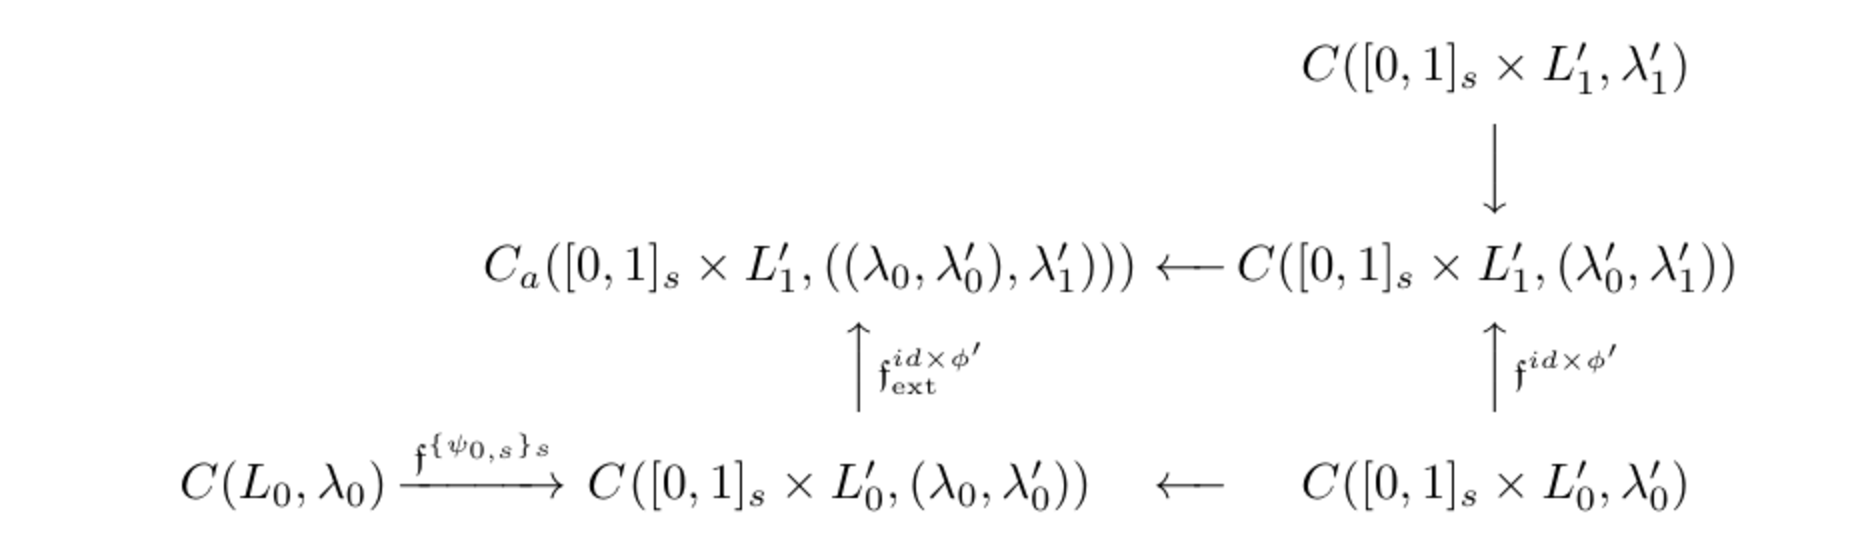
\includegraphics[width=\textwidth]{chapters/ch07-transversality/figures/phys-560-diagram-7-2-18-math-crop.png}
\par{\renewcommand{\thefigure}{7.2.18}\refstepcounter{figure}
\normalfont\bfseries 图式~\thefigure\label{diag:7-2-18}}
\end{minipage}\par\medskip
\end{lemma}

\par\noindent\textit{证明.}\quad
这是引理~\ref{lem:7-2-299} 证明的参数化版本，
也类似于第 7.2.10 小节的论述。
先说明 $\mathfrak f^{\operatorname{id}\times\phi'}$
的构造。
按照第 7.2.9--7.2.10 小节的方法定义
$C([0,1]_s\times L'_0,\lambda'_0)$
与 $C([0,1]_s\times L'_1,\lambda'_1)$。

接着使用模空间
\begin{equation}
[0,1]_s\times
\mathcal M_{k+1}^{\mathrm{main}}
((L'_1,\{J_\rho\}_\rho):\beta;
\operatorname{top}(\rho)).
\tag{7.2.302}\label{eq:7-2-302}
\end{equation}
其中
$\mathcal M_{k+1}^{\mathrm{main}}
((L'_1,\{J_\rho\}_\rho):\beta;
\operatorname{top}(\rho))$
是定义 $\mathfrak f^{\phi'}$ 时所用的模空间。
记 (7.2.302) 为
\[
\mathcal M_{k+1}^{\mathrm{main}}
(L'_1:\beta;\operatorname{top}(\rho);[0,1]_s).
\]
存在自然的评价映射
\[
\begin{aligned}
ev=(ev_1,\ldots,ev_k,ev_0)\colon\;
\mathcal M_{k+1}^{\mathrm{main}}
(L'_1:\beta;\operatorname{top}(\rho);[0,1]_s)
&\longrightarrow([0,1]\times L'_1)^{k+1}.
\end{aligned}
\]

令 $\mathcal P_i$ 为
$C([0,1]_s\times L'_0,\lambda'_0)$
中的光滑奇异链，置
$\vec{\mathcal P}=(\mathcal P_1,\ldots,\mathcal P_k)$，
并定义
\[
\begin{aligned}
&\mathcal M_{k+1}^{\mathrm{main}}
(L'_1:\beta;\operatorname{top}(\rho);[0,1]_s;
\vec{\mathcal P})\\
&\quad=
\mathcal M_{k+1}^{\mathrm{main}}
(L'_1:\beta;\operatorname{top}(\rho);[0,1]_s)
\times_{\operatorname{id}\times\phi'}
(\mathcal P_1\times\cdots\times\mathcal P_k).
\end{aligned}
\]
这里的纤维积以
$([0,1]\times L'_1)^k$ 为底，
使用 $ev_1,\ldots,ev_k$
及 $\operatorname{id}\times\phi'$。
现在利用多值截面定义其虚基本链，
再经 $ev_0$ 将它视为
$[0,1]_s\times L'_1$ 上的光滑奇异链。
于是，与第 7.2.9--7.2.10 小节一样，
得到 $C([0,1]_s\times L'_1,
(\lambda'_0,\lambda'_1))$、
其上的滤过 $A_{n',K'}$ 结构
以及滤过 $A_{n,K}$ 同态
$\mathfrak f^{\operatorname{id}\times\phi'}$，
并满足 (7.2.301.1)。

最后，将 $A_{n',K'}$ 结构和
$A_{n,K}$ 同态扩充到
$C([0,1]_s\times L'_0,(\lambda_0,\lambda'_0))$，
得到
$C_a([0,1]_s\times L'_1,
((\lambda_0,\lambda'_0),\lambda'_1))$
与 $\mathfrak f^{\operatorname{id}\times\phi'}_{\mathrm{ext}}$；
它们满足所需各项性质。$\square$
